\documentclass{article}
\usepackage{calrsfs}
\DeclareMathAlphabet{\pazocal}{OMS}{zplm}{m}{n}
\usepackage{epsfig,endnotes,xspace,hyperref,url,diagbox}
\usepackage{graphicx,subfigure,epsfig}
\pagestyle{plain}
\hyphenation{op-tical net-works semi-conduc-tor}
\renewcommand{\AA}{\mathbf{A}}
\AtBeginDocument{\let\textlabel\label}
\usepackage{calrsfs}
\DeclareMathAlphabet{\pazocal}{OMS}{zplm}{m}{n}
\usepackage{amsmath,amsthm}
\usepackage{amssymb}
\usepackage{enumerate}
\usepackage{varioref}
\usepackage{graphicx}
\usepackage{epstopdf}
\epstopdfsetup{outdir=}
\usepackage{xcolor}
\usepackage{multirow}
\usepackage{subfigure}
\usepackage{comment}
\usepackage{color}
\usepackage[utf8]{inputenc}
\usepackage[linesnumbered,ruled]{algorithm2e}
\usepackage{mathtools}
\usepackage{wrapfig}
\usepackage[noend]{algpseudocode}
\usepackage{tikz}
\usepackage{esvect}

\setlength{\evensidemargin}{0in} \setlength{\oddsidemargin}{0in}
\setlength{\textwidth}{6.5in} \setlength{\textheight}{9in}
\setlength{\topmargin}{-0.25in} \setlength{\headheight}{0in}
\newcommand{\conclusion}[1]{\vspace*{0.05in}\noindent\textbullet\textbf{\textsc{ Finding: }}{#1}\vspace*{0.05in}}

\newtheorem{theorem}{Theorem}
\newtheorem{observation}{Observation}
\newtheorem{lemma}[theorem]{Lemma}
\newtheorem{corollary}[theorem]{Corollary}
\newtheorem{definition}{Definition}
\newtheorem{fact}{Fact}
\newtheorem{example}{Example}
\newtheorem{proposition}{Proposition}

\renewcommand{\Pr}[1]{\ensuremath{\mathsf{Pr}\left[#1\right]}\xspace}
\newcommand{\DP}[1]{\ensuremath{#1\mbox{-}\mathsf{DP}}\xspace}
\newcommand{\Data}{\ensuremath{D}\xspace}

\title{Building a Classifier with Differential Privacy}

\begin{document}
\maketitle


\noindent\textbf{Due data \& time} 11:59pm on Apr. 27th, 2018.  Email your code and report to the TA (geh@purdue.edu).

\noindent\textbf{Late policy} You have three extra days in total for all your projects. Any portion of a day used counts as one day; that is, you have to use integer number of late days each time. If you exhaust your three late days, any late project won’t be graded.

\noindent\textbf{Additional instructions} (1) This project worths 10\% of the course grade, You can work as a group of two or individually.  If you work together, both students receive the same grade.  (2) The submitted homework must be typed. Using Latex is recommended, but not required.

\section{Background}
In recent years, differential privacy (DP) has been increasingly accepted as the \textit{de facto} standard for data privacy.  In a DP setting, a data curator collects personal data from each individual, and produces outputs based on the dataset in a way that satisfies differential privacy. Informally, the DP notion requires any single element in a dataset to have only a limited impact on the output.

In this project, you will get familiar with the data processing pipeline which satisfies differential privacy. The project constructs with a written task (45 pts) and a programming task (55 pts). The written task helps you to deeply understand the theoretical problem of DP. In the programming task, you are asked to implement an algorithm that takes in a sensitive dataset and outputs a noisy histogram satisfying differential privacy. More specifically, you will need to implement several functions which completes the data processing pipeline which satisfies DP.

First, let us go over the concept of Differential Privacy.

\begin{definition}[$\epsilon$-Differential Privacy] \label{def:diff}
	An algorithm $\AA$ satisfies $\epsilon$-differential privacy ($\epsilon$-DP), where $\epsilon \geq 0$,
	if and only if for any datasets $\Data$ and $\Data'$ that \emph{differ on one element}, we have
	\begin{equation}
	\forall{T\subseteq\! \mathit{Range}(\AA)}:\; \Pr{\AA(\Data)\in T} \leq e^{\epsilon}\, \Pr{\AA(\Data')\in T},\label{eq:dp1}
	\end{equation}
	where $\mathit{Range}(\AA)$ denotes the set of all possible outputs of the algorithm $\AA$.
\end{definition}

One way to understand the intuition of DP is the following ``opting-out'' analogy.  We want to publish $\AA(\Data)$, where $\Data$ consists of data of many individuals.  An individual objects to publishing $\AA(\Data)$ because her data is in $\Data$ and she is concerned about her privacy.  In this case, we can address the individual's privacy concern by removing her data from $\Data$ (or replacing her data with some arbitrary value) to obtain $\Data'$ and publishing $\AA(\Data')$.  However, achieving privacy protection by removing an individual's data is infeasible.  Since we need to protect everyone's privacy, following this approach means that we would need to remove everyone's data.  DP tries to approximate the effect of opting out, by ensuring that any effect due
to the inclusion of one's data is small.  This is achieved by ensuring that for any output, one will see the same output with a similar probability even if any single individual's data is removed (unbounded DP), or replaced (bounded DP).

\noindent\textbf{Bounded versus unbounded DP.}
 When applying DP, an important choice is the precise condition under which $\Data$ and $\Data'$ are considered to be neighboring.  In \emph{Unbounded DP}, $\Data$ and $\Data'$ are neighboring if $\Data$ can be obtained from $\Data'$ by adding or removing one element.  In \emph{Bounded DP}, $\Data$ and $\Data'$ are neighboring if $\Data$ can be obtained from $\Data'$ by replacing one element in $\Data'$ with another element.  Throughout this project, we assume bounded DP is used.
 
\noindent\textbf{Laplace Mechanism.}
To satisfy differential privacy, it requires to add some kind of noise during the process of data publishing.  The Laplace mechanism is the first and probably most widely used mechanism for DP.  It satisfies $\epsilon$-DP by adding noise to the output of a numerical function.  Specifically, to publish $f(\Data)$, one can publish $\tilde{f}(\Data)=f(\Data)+X$, where $X$ is a random variable so that
$$\forall{t}, \frac{\Pr{\tilde{f}(\Data) = t}}{\Pr{\tilde{f}(\Data') = t}} = \frac{\Pr{f(\Data) + X = t}}{\Pr{f(\Data') + X' = t}}
= \frac{\Pr{X=t-f(\Data)}}{\Pr{X'=t-f(\Data')}}  \leq e^{\epsilon},$$
where $X$ and $X'$ are drawn from the same distribution.  Let $d=f(\Data)-f(\Data')$, we need to ensure that
\begin{equation}
\forall{x},\: \frac{\Pr{X = x}}{\Pr{X' = x + d}} \leq e^{\epsilon}.  \label{eq:shift}
\end{equation}
We need to ensure that Eq.~(\ref{eq:shift}) holds for all possible $d$, and thus need the concept of the global sensitivity of $f$, which is the maximum change of $f$ between two neighboring datasets $D$ and $D'$.

\begin{definition}[Global sensitivity]
	Let $D\simeq D'$ denote that $D$ and $D'$ are neighboring.
	The global sensitivity of a function $f$, denoted by $\Delta_f$, is given below
	\begin{equation}\label{eq:globalsensitivity}
	\Delta_f  = \max_{D\simeq D'} |f(D) - f(D')|,
	\end{equation}
\end{definition}
We want to ensure that Eq.~(\ref{eq:shift}) holds for all $d \leq \Delta_f$.  In other words, the probability density function of the noise should have the property that if one moves no more than $\Delta_f$ units on the x-axis, the probability should increase or decrease by a factor of no more than $e^{\epsilon}$, i.e., if one moves no more than $1$ unit on the x-axis, the probability should change by a multiplicative factor of no more than $e^{\epsilon/\Delta_f}$.


The distribution that naturally satisfies this requirement is $\mathsf{Lap}\left(\frac{\Delta_f}{\epsilon}\right)$, the Laplace distribution,
where $\Pr{\mathsf{Lap}(\beta)=x} = \frac{1}{2\beta} e^{-|x|/\beta}$.
Note that
$$\frac{\Pr{\mathsf{Lap}(\beta) = x}}{\Pr{\mathsf{Lap}(\beta) = x + d}} \leq e^{d/\beta} \leq e^{\Delta_f/\beta} = e^{\epsilon}.$$

\begin{figure}[!htb]
	\centering
	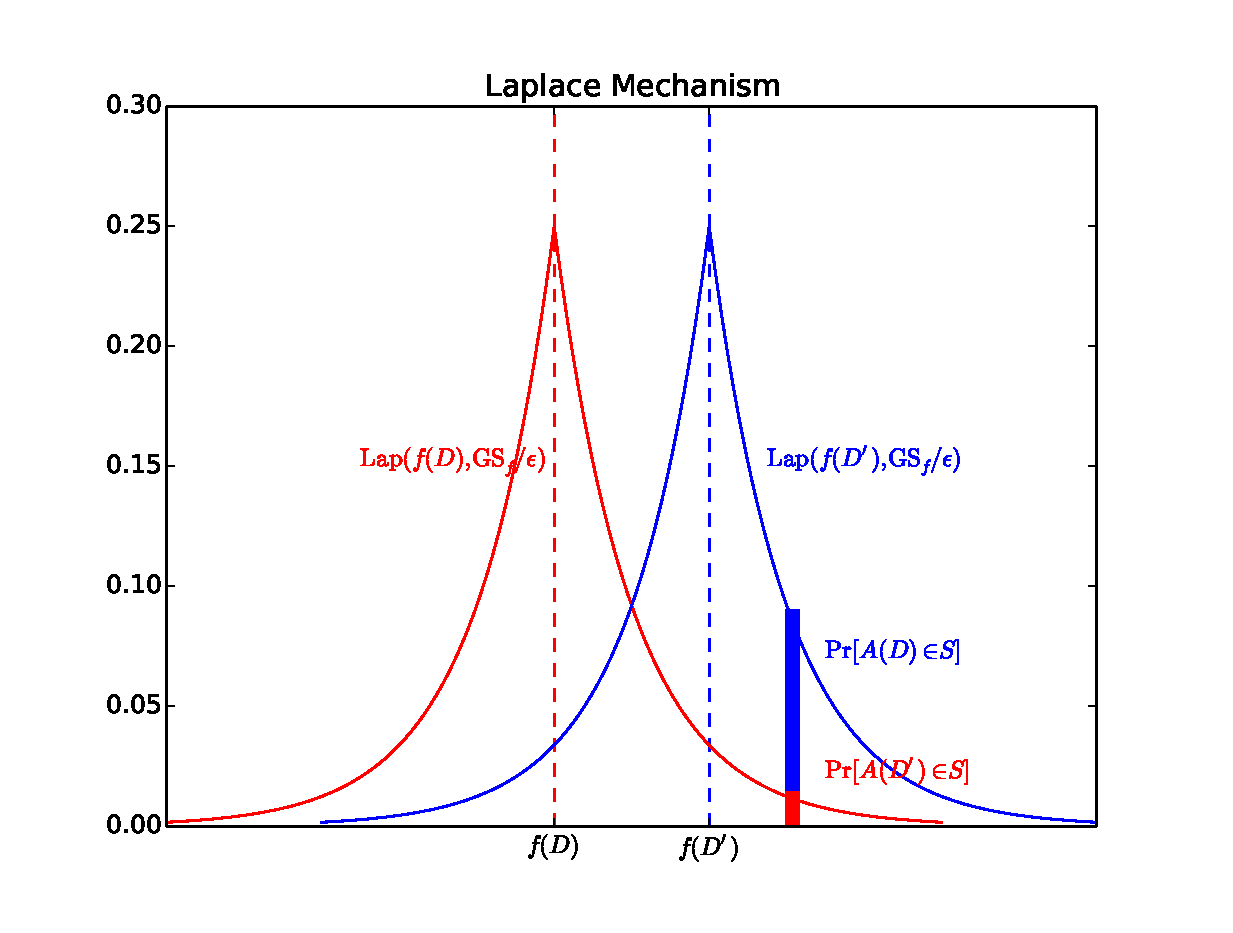
\includegraphics[width=5.0in]{lap.eps}
	\caption{Differential Privacy via Laplace Noise.\label{fig:laplaceMechanism}}
\end{figure}

\begin{theorem}[Laplace mechanism, scalar case]\label{thm:lap_scalar}
	For any function $f$, the Laplace mechanism $\AA_f(D)  = f(D)+\mathsf{Lap}\left(\frac{\Delta_f}{\epsilon}\right)$ satisfies $\epsilon$-DP.
\end{theorem}

The Laplace mechanism can also be applied to a function $f$ that outputs a vector, in which case, the global sensitivity $\Delta_f$ is the maximum $L_1$ norm of the difference between $f(D)$ and $f(D')$, i.e.:
\begin{equation}\label{eq:globalsensitivity1}
\Delta_f  = \max_{D\simeq D'} ||f(D) - f(D')||_1.
\end{equation}
And noise calibrated to the global sensitivity should be added to all components of a vector.


\begin{theorem}[Laplace mechanism, the vector case]\label{thm:lap_vector}
	The Laplace mechanism for a function $f$ whose value is a $k$-dimensional vector, defined below, satisfies $\epsilon$-DP.
	\begin{equation*}
	\AA_f(D)  = f(D)+\langle X_1, X_2, \cdots, X_k\rangle,
	\end{equation*}
	where $X_1, X_2, \cdots, X_k$ are i.i.d. random variables drawn from
	$\mathsf{Lap}\left(\frac{\Delta_f}{\epsilon}\right)$.
\end{theorem}


Sometimes, the algorithm is complicated and has multiple steps.  To argue the whole algorithm is private, it is easy to proof each step is private, and use the following composition theorem:

\begin{theorem}[General Sequential Composition] \label{lem:gscomp}
	Let $\mathcal{A}_1, \mathcal{A}_2, \cdots, \mathcal{A}_k$ be $k$
	algorithms (that take auxiliary inputs) that satisfy $\epsilon_1$-DP, $\epsilon_2$-DP, $\cdots$,
	$\epsilon_k$-DP, respectively, with respect to the input dataset.
	Publishing %$\mathbf{t} = \tuple{t_1,t_2,\cdots,t_k}$, where
	$$\mathbf{t} = \langle t_1,t_2,\cdots,t_k\rangle, \mbox{ where } t_1=\mathcal{A}_1(D), t_2=\mathcal{A}_2(t_1,D), \cdots, t_k=\mathcal{A}_k(\langle t_1,\cdots,t_{k-1}\rangle,\Data)$$
	%the outputs of all $k$ algorithms on an input $\Data$
	satisfies $(\sum_{i=1}^k \epsilon_i)$-DP.
\end{theorem}

%\begin{proposition}[Sequential Composition.] \label{lem:comp}
%	Let $\mathcal{A}_1, \mathcal{A}_2, \cdots, \mathcal{A}_k$ be $k$
%	algorithms that satisfy $\epsilon_1$-DP, $\epsilon_2$-DP, $\cdots$,
%	$\epsilon_k$-DP, respectively.  Publishing the outputs of all $k$
%	algorithms on an input $\Data$ satisfies $(\sum_{i=1}^k
%	\epsilon_i)$-DP.
%\end{proposition}

Note that each of the $\mathcal{A}_i$ will read the whole dataset.  If some operation only touches the noisy result, it will not contribute to $\epsilon$. 

\section{Written Tasks (45 pts total)}
To understand DP better, you are asked to answer the following theoretical problems.  Note that all the questions are based on the bounded DP definition.
 
\begin{enumerate}

%	\item Given a random function that generates a variable from uniform distribution within range $(0,1)$ each time, say $uni()$, describe (using pseudo-code) a simple function to generate variables from Laplace distribution with mean $0$ and scale $b$, i.e., $lap\left(b\right)$.
	
	\item Suppose that all the $n$ values are in the range $[a,b]$, what is the sensitivity for the following functions?  (Hint: The questions on the slides are for unbounded DP.) (1) sum, (2) mean, (3) median. (\textbf{9 pts})
	
	\item Suppose that all the $n$ values are either $a$ or $b$.  Suppose your DP algorithm outputs the number of $a$ values and $b$ values, respectively (with Laplace mechanism under privacy budget $\epsilon$), and you now calculate the mean of these $n$ values.  What is the variance of this estimation? (Hint: Get familiar with Laplace distribution on wiki.) (\textbf{6 pts})
	
	\item Suppose that the $n$ values each has two attributes, age and gender.  You are going to publish a histogram (with Laplace mechanism and $\epsilon$) of both attribute, with age bucketized into $[0-49]$ and $[50-100]$ (so there will be four numbers for: male-$[0-49]$, male-$[50-100]$, female-$[0-49]$, female-$[50-100]$).  Now you want to estimate the number of male users, what is the variance of this estimation?  What is the variance if you just use the gender attribute and ignore age when you publish the histogram?  If each value has $d$ binary attributes, what is the size of your histogram? (\textbf{10 pts})
	
	\item Suppose that all the $n$ values are in the range $[a,b]$, and your task is to publish the $25$th, $50$th, and $75$th percentiles (assume $n>100$).  Now you are given an algorithm that adds independent Laplace noise $\mathsf{Lap}\left(\beta_{25}\right)$, $\mathsf{Lap}\left(\beta_{50}\right)$, and $\mathsf{Lap}\left(\beta_{75}\right)$, to the real answers, respectively ($\beta_{25}<\beta_{50}<\beta_{75}$).  Your task is to find out (1) what is the sensitivity of this problem, (2) what is the final minimal $\epsilon$ this algorithm can achieve? (Hint: You should argue by a proof starting from Definition~\ref{def:diff}.) (\textbf{10 pts})
	
	\item If there is no public dataset available, and you instead use $10\%$ of your sensitive data, sampled randomly, to find the desired histogram, without differential privacy.  The remaining $90\%$ of data is used to calculate the exact values in each cell of the histogram (and then add Laplace noise $\mathsf{Lap}\left(\frac{1}{\epsilon}\right)$).  What will be the worst case  $\epsilon$ for the whole process? (Hint: Look at each step separately, start from Definition~\ref{def:diff} with the histogram structure as the output; the sample probability for each value is thus $10\%$.) (\textbf{10 pts})
	
\end{enumerate}

%\noindent\textbf{Task 2:} Prove Theorem~\ref{thm:lap_scalar}.  (Hint: the answer should be direct from the background description.)
%
%\noindent\textbf{Task 3:} Prove Theorem~\ref{thm:lap_vector}.  (Hint: )
%
%\noindent\textbf{Task 4:} Prove Proposition~\ref{lem:comp}.  (Hint: start from Definition~\ref{def:diff}.)

%\noindent\textbf{Task 5:} A brief report of the programming task described below.  The report should describe your algorithm, the reason for your design, and the argument why your algorithm is $\epsilon$-DP.  
%To prove DP, you can use sequential composition.  But make sure to mention clearly in which step your algorithm reads any data, what $\epsilon$ is used to add noise right after that step.

\section{Programming Tasks (55 pts total)}

A data scientist in your company wants to share data with other companies by using a data processing pipeline. What the collaborating companies want is a classifier: they want to predict some behavior of their incoming customer.  And in this specific task, they want to learn whether the customer is earning over $50K$ dollars a year. As the chief privacy officer, you understand that sharing raw data is dangerous, and suggest to enhance the existed data processing pipeline by implementing an algorithm which publishing a differentially private histogram.

%The data itself is high-dimensional -- some (occupation) may be highly correlated to their annual income, while some (workclass) may be less informative.  
%Therefore, you want to select only related features with appropriate granularity, and publish the histogram.
%Once the ``noisy'' histogram is handed to the collaborating companies, they can then train whatever model they would like to use.
%Luckily, you also found a public dataset of the same form, and it seems that dataset is contributed from the similar population -- yours is from Indiana residents and the public one is from Illinois.
%So your goal is to select features and granularities based on your experience with the public dataset, and implement an algorithm that given your sensitive dataset outputs a noisy histogram satisfying differential privacy.


\subsection{Dataset}
We use the UCI Machine Learning Adult Data Set (\url{https://archive.ics.uci.edu/ml/datasets/adult}) to predict whether the income of an individual exceeds \$50K/yr based on census data. Also known as "Census Income" dataset. The dataset can be downloaded from \url{https://archive.ics.uci.edu/ml/machine-learning-databases/adult/adult.data}.

\subsection{Differential Private Data Processing Pipeline}
The sample code of the Data Processing Pipeline consists of 6 steps which are briefly described in the following:
\begin{enumerate}
    \item \textbf{Parse the raw dataset}\par
        The program loads the UCI Adult data (CSV format) into the memory.
    \item \textbf{Project the raw dataset into a histogram} \par
        Each record in the dataset has multiple attributes e.g., numerical attribute such as age and categorical attributes such as gender and marriage statues, etc.  To project the dataset into a histogram, you need to select some buckets for each attribute.  For example, the attribute marital-status has multiple different possible values: Married-civ-spouse, Divorced, Never-married, Separated, Widowed, Married-spouse-absent, Married-AF-spouse.  You can bucketize this attribute into `single' and `married'.  You can also have more buckets to carry more information, such as `never-married', `divorced', `divorced-marry-again', etc.  Furthermore, you can have unbalanced buckets such as `divorced' and `other'.  If you want to ignore this attribute completely, you can have one `any' bucket.  The cells in the histogram are the Cartesian product of all buckets for all attributes.  Once you have the cells, you can simply count the number of records for each cell (each record can only belong to one cell).
    \item \textbf{Add noise to the histogram}
    \item \textbf{Generate a synthetic dataset from the histogram}\par
        Suppose the generated histogram has $N$ cells. Each cell represents a list of attributes and has count $c_i$, where $1\leq i \leq n$. The synthetic dataset should contains $c_i$ records for the $i$-th cell.
    \item \textbf{Train the classification model based on the re-generated data}\par
        Split the synthetic dataset into training and test sets with 80/20. Train a logistic regression classification model with the split training data.
    \item \textbf{Test the model prediction accuracy}\par
        Evaluate the model prediction accuracy against the test data and output the accuracy score.
\end{enumerate}

The sample code provides steps 1 to 6, but it is not differential private. \textbf{Your task is to complete steps 2 and 3} to make the histogram to be differential private and also achieve a reasonable prediction accuracy. More specifically, after studying the dataset, you found three attributes, age, salary, and investment gain, are informative for annual income. And the average annual income for 40-year-olds are highest. You can keep the unbalanced buckets `$[40-50]$' and `other' for age, and try different precision for salary and investment. By running at least $10$ times for different $\epsilon$ value, find which histogram performs best. Regard to step 3, The noise you added in the histogram should satisfying the definition of bounded DP. 

\subsection{Programming Environment}
Please use python 3 to implement your algorithm.  You are allowed to use following python non-default packages: sklearn, pandas, numpy, scipy, and pickle (current version).  Please email TA if your code needs to use other packages and explain the reason.

\begin{itemize}
    \item \textbf{What's in the sample code?}
        \begin{itemize}
            \item \texttt{exp.py} The main script for running data processing pipeline. You should not make any changes to this file.
            \item \texttt{hist.py} You should make your implementation in this file. Make sure that your code does not change the function interface of \texttt{project\_hist} and does not generate any command line output. You are free to add additional functions.
        \end{itemize}
    \item \textbf{How to run the sample code?}
        Download the sample code and adult data. Put them under the same directory. Install packages in local if you do not have.
        $$\texttt{pip3 install --user sklearn pandas numpy}$$
        You can choose install package globally, requiring root privilege.
        $$\texttt{sudo pip3 install sklearn pandas numpy}$$
        To run the code, use the following command
        $$\texttt{python3 exp.py --epsilon=0.1 --file=adult.data.txt}$$
        For details of the sample code, please read the source code or check the command $$\texttt{python3 exp.py --help}$$
\end{itemize}

\section{Submission}
You should submit your implementation code \texttt{hist.py} and the project report to the TA. The project report should include both the written task and the description of your implementation.

\section{Grading policy:}
\begin{enumerate}
    \item \textbf{Written Tasks}: \textbf{45 pts}
    \item \textbf{Programming Tasks}: \textbf{55 pts}\par
        Given the histogram, we will synthesize a dataset and use logistic regression to train a model, which is used to test for mis-classification rate.  The mis-classification rate is the average for three epsilon values: 0.1, 0.5, 1.0 (run 10 times for each value). Your grade will be depended on the prediction accuracy and the DP sanctification.
        
        Here are the specific distribution of the points:
        \begin{itemize}
            \item A brief report of the programming task is required.  The report should describe your algorithm, the reason for your design, and the argument why your algorithm is $\epsilon$-DP. (\textbf{10 pts})
            \item As long as your algorithm works, you receive the implementation points (\textbf{10 pts})
            \item As long as your algorithm satisfies DP (you should explain this in your report), you receive the privacy points. (\textbf{10 pts})
            \item As long as your algorithm can beat majority vote (mis-classification rate $<25\%$), you receive the base points (\textbf{10 pts}).  Note that if the algorithm is not private, you cannot receive the points below.
            \item As long as your algorithm can achieve mis-classification rate $<20\%$, you receive the advanced points. (\textbf{10 pts})
            \item As long as your algorithm beat algorithms from other students, and the non-private example, you receive the top points. (\textbf{5 pts})	
        \end{itemize}
\end{enumerate}

\end{document}
